\section{NNTD}
\subsection{What do we want to measure?}
\begin{frame}{Our goal}
\begin{center}
\textbf{At first}

Many fit individuals with different traits
\end{center}
\end{frame}

\begin{frame}{Our goal}
\begin{center}
\textbf{At last}

Find the combination of traits that forms the most fit individual.
\end{center}
\end{frame}

\begin{frame}{Traits}
\begin{center}
  What traits can an artificial intelligent player have in the cell phone game Snake?
  \begin{figure}[p]
  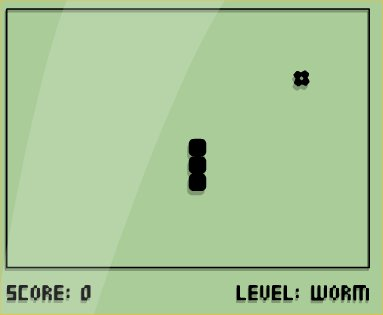
\includegraphics[width=0.7\textwidth]{images/snake.jpg}
  \end{figure}
  \end{center}
\end{frame}

\begin{frame}{Traits}
\begin{center}
  When do two neural networks have different traits in general?
  \end{center}
\end{frame}

\begin{frame}{NNTD}
\begin{center}
  Input: A set of neural networks.\\
  Output: A diversity measurement based on difference in \emph{traits}.
\end{center}
\end{frame}

\begin{frame}{NNTD}
\begin{center}
Calculate a large amount of random inputs (a-tuples) for the neural network architecture used
 \begin{figure}[p]
  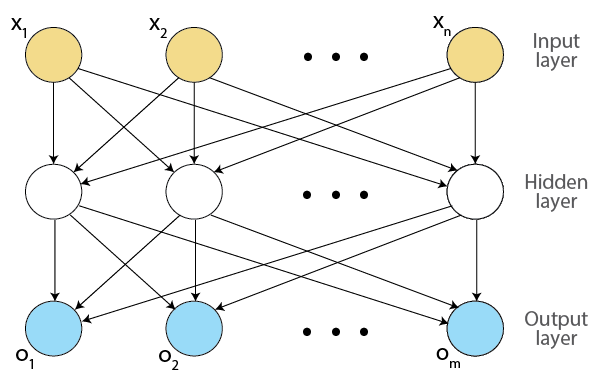
\includegraphics[width=0.7\textwidth]{images/neuralnetwork.png}
  \end{figure}
\end{center}
\end{frame}

\begin{frame}{NNTD}
\begin{center}
For each input:
  \begin{itemize}
      \item Calculate the output of all neural networks.
  \end{itemize}
   \begin{figure}[p]
  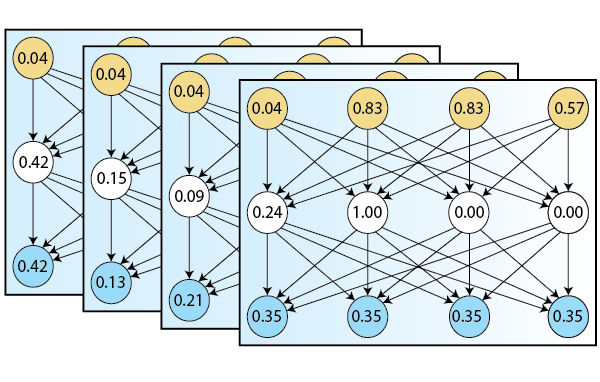
\includegraphics[width=0.7\textwidth]{images/neuralnetworkvalues.png}
  \end{figure}
\end{center}
\end{frame}

\begin{frame}{NNTD}
\begin{center}
For each input:
  \begin{itemize}
	  \item Distribute the neural networks into species based on their output.
  \end{itemize}
     \begin{figure}[p]
  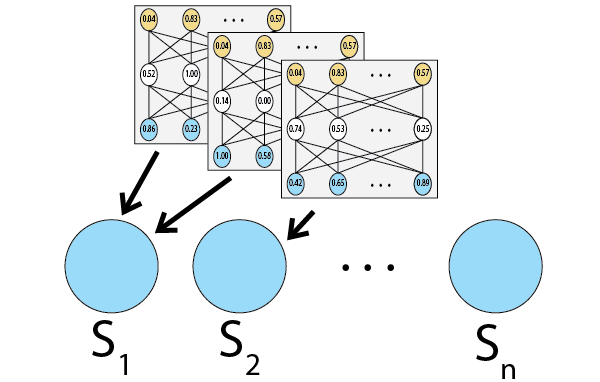
\includegraphics[width=0.7\textwidth]{images/speciesnn.png}
  \end{figure}
\end{center}
\end{frame}

\begin{frame}{NNTD}
\begin{center}
For each input:
  \begin{itemize}
	  \item Calculate Simpson's Diversity Index based on the size of each species.
  \end{itemize}
     \begin{figure}[p]
  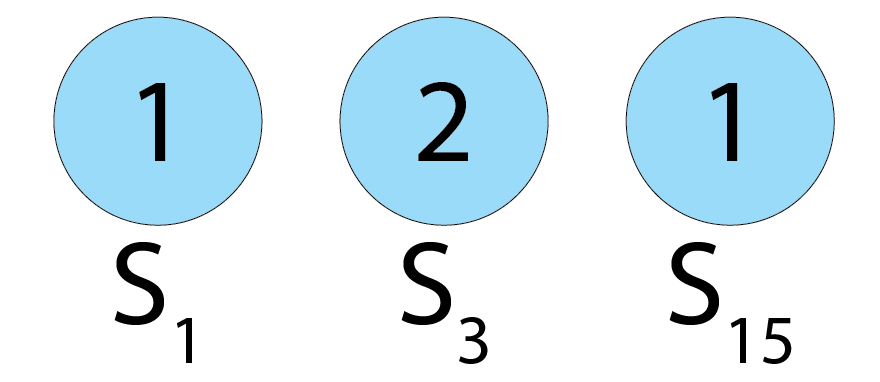
\includegraphics[width=0.4\textwidth]{images/speciessize.png}
  \end{figure}
\end{center}
\end{frame}

\begin{frame}{NNTD}
\begin{center}
\textbf{NNTD:}\\
The average Simpson's Diversity Index for all random inputs.
\end{center}
\end{frame}

\begin{frame}{Simpson's Diversity Index}
\begin{center}
  \begin{figure}[p]
  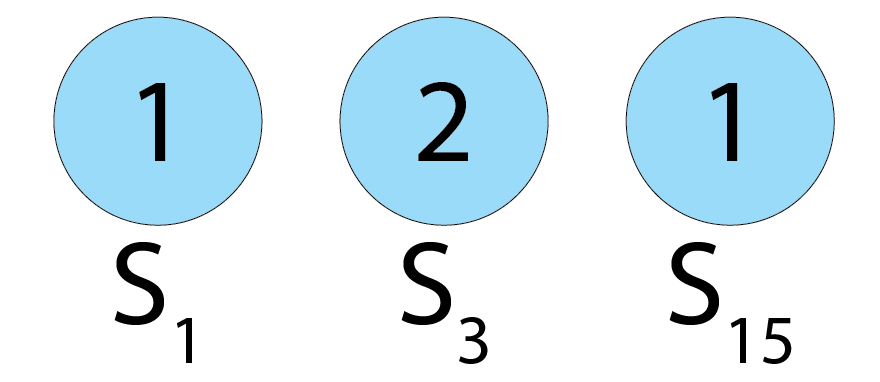
\includegraphics[width=0.4\textwidth]{images/speciessize.png}
  \end{figure}
  \begin{equation}\label{eq:nntd}
  D_r = 1 - \frac{\sum_{q \in \nemptyspeciesf{r}}\left(\sizeof{q}\left(\sizeof{q} - 1\right)\right)}{\indsetl\left(\indsetl - 1\right)}
\end{equation}
\end{center}
\end{frame}

\begin{frame}{Distribution of neural networks into species}
\begin{center}
Given neural network $f$ and input $\ran = (0.04, 0.83, 0.83, 0.57)$
  \begin{figure}[p]
  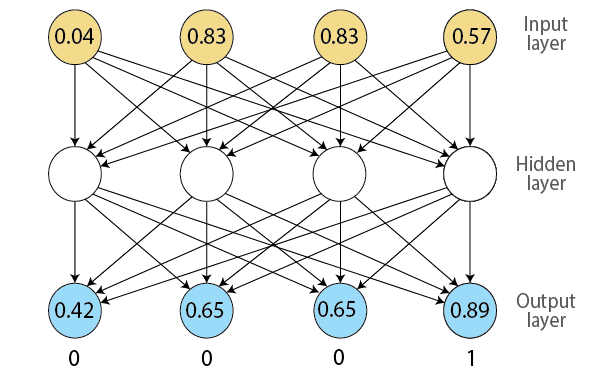
\includegraphics[width=0.75\textwidth]{images/nntdexample1.png}
  \end{figure}
We say that $f \in \speciesi{1}{\ran}$, because binary $\texttt{0001}$ is $1$ in decimal.
\end{center}
\end{frame}

\begin{frame}{Distribution of neural networks into species}
\begin{center}
Given neural network $f$ and input $\ran = (34, -5.7, 0, -4)$
  \begin{figure}[p]
  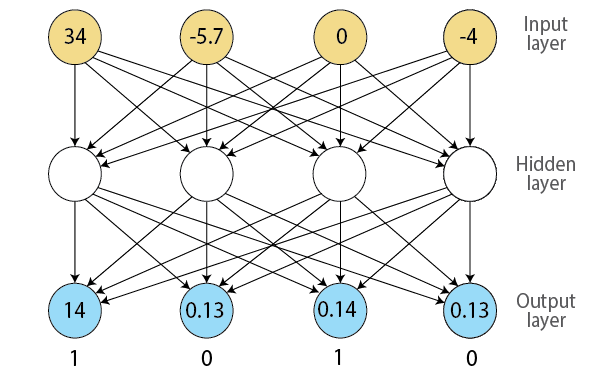
\includegraphics[width=0.75\textwidth]{images/nntdexample2.png}
  \end{figure}
We say that $f \in \speciesi{10}{\ran}$, because binary $\texttt{1010}$ is $10$ in decimal.
\end{center}
\end{frame}

\begin{frame}{Distribution of neural networks into species}
\begin{center}
Given neural network $f$ and input $\ran = (1, -1, 0, -1)$
  \begin{figure}[p]
  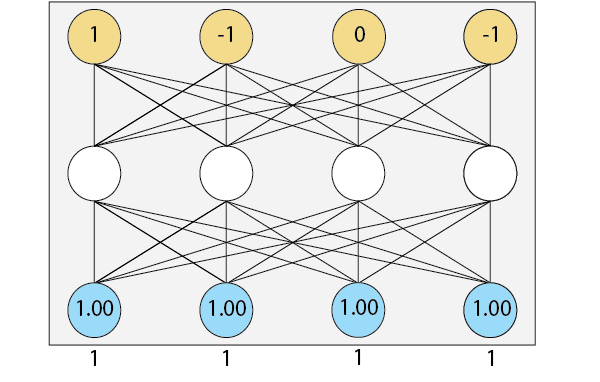
\includegraphics[width=0.75\textwidth]{images/nntdexample3.png}
  \end{figure}
We say that $f \in \speciesi{15}{\ran}$, because binary $\texttt{1111}$ is $15$ in decimal.
\end{center}
\end{frame}

\begin{frame}{Formally}
\begin{center}
If $b_{m}b_{m-1}\dots b_1$ is the binary representation of a number $i$, we define the species \speciesi{i}{\ran} to contain any neural network $\ind \in \indset$, that given $\ran$ as input satisfies
\begin{equation}
  \forall j \in \set{m, m-1, \dots, 1} \left(b_j \rightarrow (\nnout_j = h) \wedge \neg b_j \rightarrow (\nnout_j < h)\right)
\end{equation}
where $h = \max\set{\nnout_1, \nnout_2, \cdots, \nnout_b}$
\end{center}
\end{frame}


